An accurate and real-time backscatter-cancelling lighting system must consider five main factors: (a) precise backscatter particle segmentation even in varying environmental conditions by mapping the exact backscatter positions to aid in (b), the accurate projection of the backscatter cancelling light patterns, ensuring the whole scene except backscatter is lit, (c) low system latency by minimising the time it takes between frame capture and the light pattern projection, ensuring the projection is still correct even with fast-moving backscatter, interlinked with (d), adequate system throughput with parallel processing to increase system responsiveness for reaching the low latency goal, and finally, (e) the ability to control and establish the system frame rate to ensure system predictability.

This section, gathers background information on the five system factors, beginning with an investigation of previous work on this project. Then exploring work related to underwater imaging for precise environmental analysis. Finally, a study on computer systems and architectures for this project and a summary of all aspects concludes the section.

\subsection{Previous Work in Underwater Anti-Backscatter Lighting Systems}
\label{prevwork}

Previous work on this project in \cite{katieshepherdMachineVisionBased2023} by Shepherd introduces a backscatter-cancelling lighting system with goals similar to what this paper proposes. Shepherd presents a two-stage process, which is fundamental to their system, illustrated in Figure \ref{fig:shepherd_system_stages}. The first stage is `detection', where the specialised projector illuminates the whole scene with a low-brightness, solid white output intending to forcefully induce backscatter particles for detection with machine vision techniques. The second stage is `pattern projection', where the system overlays black ellipses called `holes' at the positions of detected backscatter particles over a full-brightness, solid white projection to eliminate backscatter.

\begin{figure}[H]
    \centering
    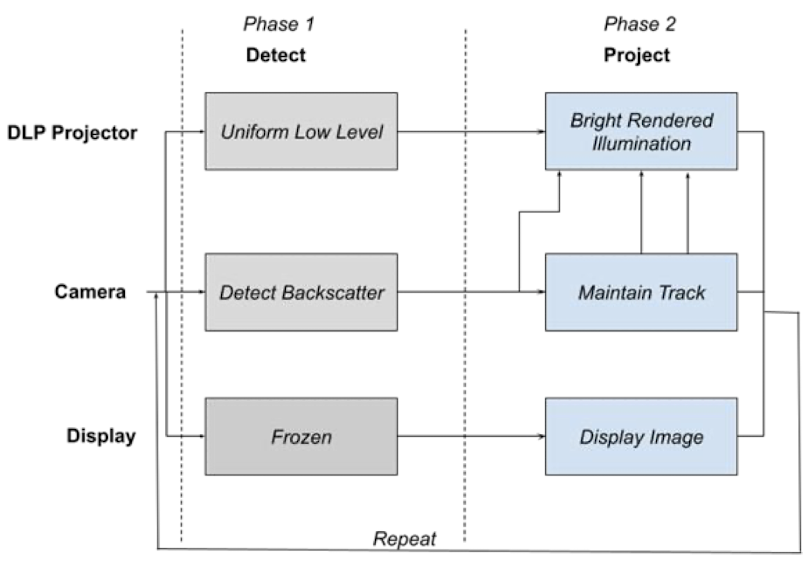
\includegraphics[width=0.7\textwidth]{assets/shepherd_fig6_system.png}
    \caption{The high-level system stages from \cite{katieshepherdMachineVisionBased2023}.}
    \label{fig:shepherd_system_stages}
\end{figure}

Shepherd designs the backscatter segmentation system based on a simple blob detection algorithm \cite{opencvOpenCVCvSimpleBlobDetector}, where the term `blob' denotes a group of connected pixels in a binary image. By applying several thresholds, the algorithm first converts the input image into a binary representation to then extract connected pixels and calculate the centre positions of each. After grouping the centre positions from the binary images, the algorithm finally estimates the final centroid and radii for each `blob'. While this blob detection algorithm benefits from a computationally simple approach, it suffers from a drastic drawback as Shepherd describes ``at least one property needs to be shared between the blobs such as size or shape to allow for the isolation of these blobs''. The underwater environment is unpredictable, where backscatter particles can never share the same characteristics, making this approach unviable.

\subsection{Automotive Headlights for Illumination Through Rain and Snow}
\label{autolights}

Similar to the underwater backscatter that this paper explores and attempts to eliminate, the work in \cite{decharetteFastReactiveControl2012} by De Charette et al. outlines an automotive headlight system to illuminate around the backscatter caused by rain and snow whilst driving. The parallax issue observed by Shepherd, where the displacement between the camera's and projector's viewpoint causes a perceived offset in object positioning, is resolved in De Charette et al. using a beamsplitter arrangement, illustrated in Figure \ref{fig:beamsplitter_system}, such that the incident visual beam is split 50:50 between the projector and camera, thus eliminating parallax displacement by co-location.

\begin{figure}[H]
    \centering
    \begin{subfigure}{.49\textwidth}
        \centering
        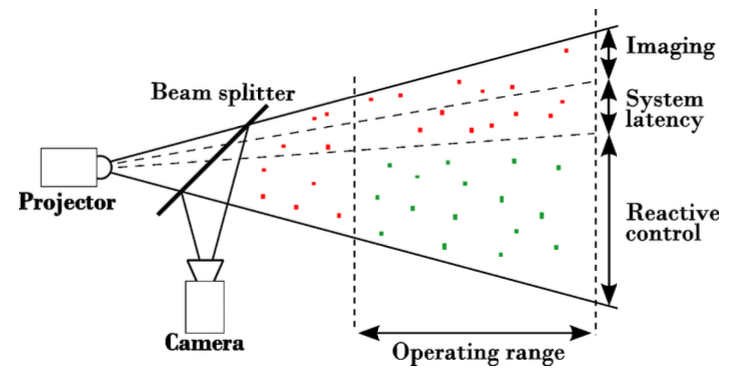
\includegraphics[width=1\textwidth]{assets/beamsplitter_automotive_system.png}
        \caption{}
        \label{fig:beamsplitter_system}
    \end{subfigure}
    \hfill
    \begin{subfigure}{.49\textwidth}
        \centering
        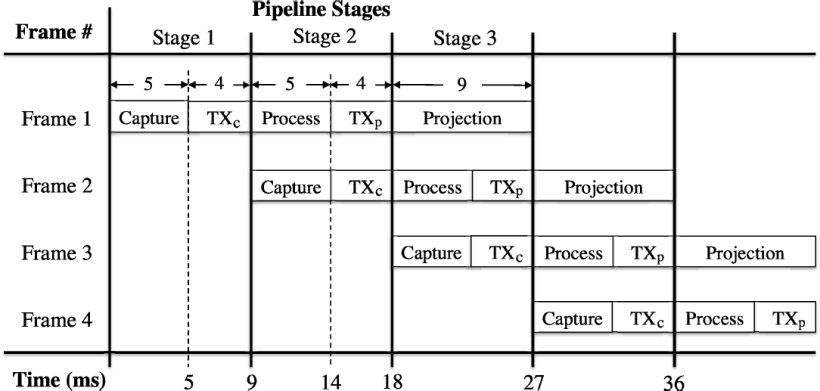
\includegraphics[width=1\textwidth]{assets/cmu_auto_pipeline.png}
        \caption{}
        \label{fig:cmu_auto_pipeline}
    \end{subfigure}
    \caption{From \cite{decharetteFastReactiveControl2012}: (\ref{sub@fig:beamsplitter_system}) The system configuration including a beamsplitter for parallax elimination through co-location, (\ref{sub@fig:cmu_auto_pipeline}) the parallel pipeline stages for their system.}
    \label{fig:decharette}
\end{figure}

The automotive backscatter-cancelling headlight system utilises an image processing pipeline that applies a background subtraction, albeit not specifying the exact method, followed by blurring and thresholding to isolate the bright water spots. The system employs the connected-components algorithm to segment the backscatter particles, this algorithm scans an image to group its pixels into components based on pixel connectivity, i.e., all pixels in a connected component share similar pixel intensity values and are in some way connected \cite{robertfisherConnectedComponentsLabeling2003}. Unlike Shepherd's system which employs a blob detection algorithm, this system is resilient to unique backscatter particle characteristics, allowing for segmentation regardless of fixed parameters despite also being a computationally simple approach. However, the connected-components algorithm may be inherently limited when given low-quality input images as it may not correctly connect pixels due to distortion and noise.

Although not specifying the exact methods, the automotive system in De Charette et al. employs backscatter particle tracking with a predictive algorithm to project backscatter-cancelling light patterns by accounting for the movement during the system processing period, denoted by the system latency time. Due to the linear and vertical movement of rain and snowfall, one can assume they are using a simple linear interpolative approach with the assumption the particles are moving at a constant speed, to predict the future particle position. To increase system throughput, the work in De Charette et al. proposes a three-stage parallel processing pipeline, illustrated in Figure \ref{fig:cmu_auto_pipeline}. Stage 1 represents the task of capturing the frame from the camera, with $TX_c$ denoting the image data transfer from the camera to the computer. Stage 2 represents the image processing steps, with drop detection, prediction, and projection pattern generation, with $TX_p$ denoting the computer-to-projector data transfer. The third and final stage represents the refresh time of the projector. This system, once primed, will run with a three-frame latency: as the $n^{th}$ frame is being captured, the $n^{th} - 1$ frame is being processed, and the $n^{th} - 2$ frame is being projected. With this fixed latency mitigated by the predictive functionality.

The system in De Charette et al. takes, on average across 5500 frames, \SI{4.214}{\milli\second} to transfer data from the camera to the host computer, a \SI{3.2}{\giga\hertz} Intel Xeon processor with \SI{8}{\giga\byte} of RAM running Windows Vista 64-bit, \SI{4.081}{\milli\second} to process the image, \SI{4.214}{\milli\second} to send the data to the projector, and \SI{9}{\milli\second} for the projector to output. Thus, total system latency is \SI{21.51}{\milli\second}, with an accuracy of 68.9\% for rain. The work in \cite{tamburoProgrammableAutomotiveHeadlights2014} by Tamburo et al. expands on the system by De Charette et al. with a more powerful desktop PC for image processing and an FPGA-based controller for the specialised projector. This system achieves an average frame processing time of \SI{0.3}{\milli\second}, with a total response time ranging between \SI{1}{\milli\second} to \SI{2.5}{\milli\second}.

\subsection{Underwater Gas Seepage Bubble Quantification for Environmental Analysis}
\label{gasquant}

Aside from the work by Shepherd, De Charette et al., and Tamburo et al., public documentation of research related to real-time efforts for underwater backscatter-cancelling lighting systems is non-existent. However, numerous environmental analysis fields rely on highly specialised and precise systems for quantifying underwater bubbles to investigate gas seepages from the sea floor. As underwater backscatter can comprise a mixture of compositions, ranging from bubbles and sand to all sorts of marine debris, it will be beneficial to explore gas escape measurement and monitoring systems as they require high precision, extensive range, strong anti-interference, and low cost under complex underwater conditions \cite{zhangUnderwaterBubbleEscape2023}.

The work in \cite{thomanekAutomatedGasBubble2010} by Thomanek et al. presents a novel approach for a highly precise automated gas bubble imaging system that employs the Canny edge detection algorithm. The Canny algorithm, which prefers a single channel (greyscale) input, first smoothens the input using Gaussian convolution before comparing each pixel's values relative to its neighbours such that when the gradient is above a certain threshold, it sets the bordering pixel a value of `1', otherwise `0', resulting in the formation of edges around objects \cite{cannyComputationalApproachEdge1986a}. In contrast to the system by Shepherd, the Canny approach in Thomanek et al. works around the object characteristics limitation of the simple blob detection algorithm.

The paper compares the Canny algorithm approach with the simple image binary thresholding method, where only the pixels with intensities within a certain threshold are passed through, ultimately establishing Canny as the more accurate choice for segmentation, even in areas of uneven illumination, illustrated in Figure \ref{fig:canny_segmentation_compare}. However, the drawbacks of the Canny approach, as highlighted by Thomanek et al., include a significant increase in computing time, and the necessity for implementing morphological techniques to address bubble transformation issues such as expansion and contraction during segmentation. Nevertheless, considering the advancements in computing power over the past 14 years since this paper was published, modern computers should now be easily capable of handling this workload with relative ease.

\begin{figure}[H]
    \centering
    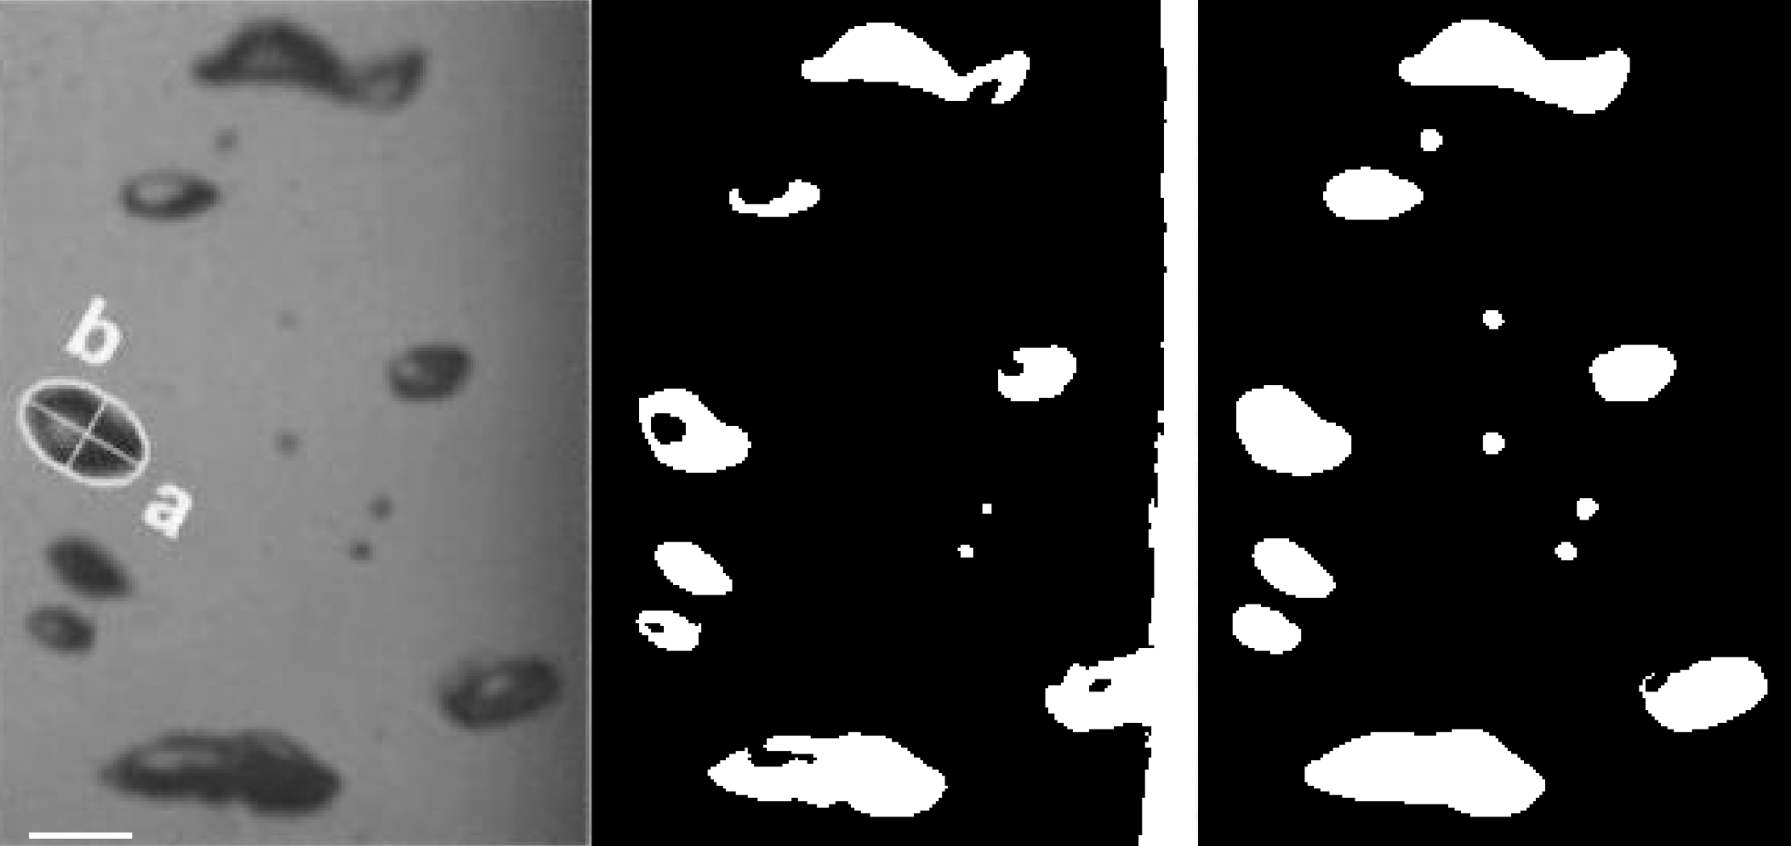
\includegraphics[width=0.7\textwidth]{assets/bubble-segmentation-canny-thresholding.png}
    \caption{From \cite{thomanekAutomatedGasBubble2010}, the original input frame in the left-most image, bubble segmentation using simple binary thresholding in the middle, and bubble segmentation using the Canny edge detection algorithm in the right-most image.}
    \label{fig:canny_segmentation_compare}
\end{figure}

While this paper by Thomanek et al. provides valuable insight and serves as an excellent starting point, it primarily emphasises system construction and quantifying gas flux measurements. Consequently, certain crucial details, such as the precise methodology employed for achieving the highlighted bubbles post-Canny segmentation in Figure \ref{fig:canny_segmentation_compare}, receive less attention. However, one can infer that Thomanek et al. may have employed a logical algorithm to fill closed-loop edges. The study by Zelenka in \cite{zelenkaGasBubbleShape2014a} builds upon the foundational system by Thomanek et al. aiming to address the sporadic false detection issue that is inherent in the Canny edge detection algorithm, introducing robust algorithms capable of achieving precise bubble stream quantification with accurate bubble fitting.

Zelenka introduces a snake-based active contour model developed by Kass et al. in \cite{kassSnakesActiveContour1988} for a more stable and precise method for bubble detection. As explained by Kass et al., a snake embodies an energy-minimising spline that's guided by external forces and influenced by image characteristics that collectively drive the snake towards prominent features within the image, such as lines and edges, all while the snake dynamically adheres to nearby edges due to the active contour model. The classic snake method, illustrated in Figure \ref{subfig:classic_snake}, uses a bounding box from the baseline localisation for initialisation, shown in blue, from which the snake algorithm optimises with each iteration on a low-quality image sequence. The figure exemplifies the unreliability of the classic snake method due to light areas within the centre of the bubble, as the red outline borders this region instead of the bubble itself. Zelenka, therefore, introduces a novel enhancement to the classic snake method to improve performance in varying lighting conditions by utilising gradient information of an image to compute external energy terms that guide the snake.

Zelenka compares all of these bubble segmentation methods using a sequence of 20 GoPro-captured images, with circa 10 bubbles visible per frame and manual ground truth. The results, illustrated in Figure \ref{fig:zelenka_performance}, show a clear improvement across all methods compared to the baseline Canny approach, which achieved a detection rate of 77.3\%. The classic snake approach achieved the best detection rate of 89.7\% and the gradient-snake achieved 89.3\%.

\begin{figure}[H]
    \centering
    \begin{subfigure}{.49\textwidth}
        \centering
        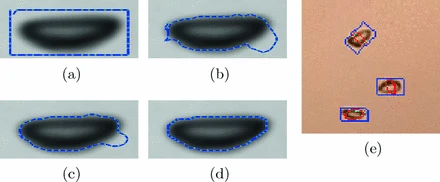
\includegraphics[width=1\linewidth]{assets/classic_snake.png}
        \caption{Classic snake algorithm.}
        \label{subfig:classic_snake}
    \end{subfigure}
    \hfill
    \begin{subfigure}{.49\textwidth}
        \centering
        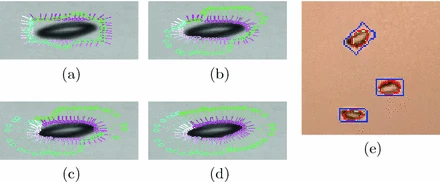
\includegraphics[width=1\linewidth]{assets/gradient_snake.png}
        \caption{Gradient-based snake algorithm.}
        \label{subfig:gradient_snake}
    \end{subfigure}
    \caption{The classic snake method in (\ref{sub@subfig:classic_snake}) and the gradient snake method in (\ref{sub@subfig:classic_snake}) from \cite{zelenkaGasBubbleShape2014a}. Sub-subfigures from (a) to (d) for both methods show every third step in the snake optimisation process, and (e) shows the final result.}
    \label{fig:snake_methods}
\end{figure}

\begin{figure}[H]
    \centering
    \begin{subfigure}{.40\textwidth}
        \centering
        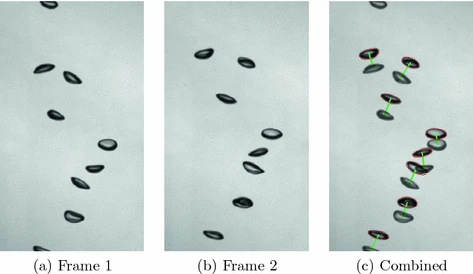
\includegraphics[width=1\textwidth]{assets/zelenka_system.png}
        \caption{}
        \label{fig:zelenka_system}
    \end{subfigure}
    \hfill
    \begin{subfigure}{.55\textwidth}
        \centering
        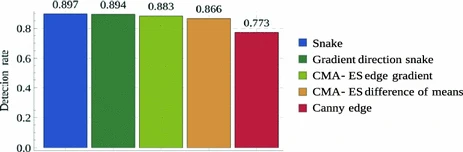
\includegraphics[width=1\textwidth]{assets/zelenka_performance.png}
        \caption{}
        \label{fig:zelenka_performance}
    \end{subfigure}
    \caption{From \cite{zelenkaGasBubbleShape2014a}: (\ref{sub@fig:zelenka_system}) demonstration of the system across two subsequent frames at 100 FPS, with the red border denoting bubble detection and the green lines denoting bubble tracking, (\ref{sub@fig:zelenka_performance}) a comparison of bubble detection rates for different segmentation approaches.}
    \label{fig:zelenka}
\end{figure}

Thomanek et al. introduced a novel approach for bubble tracking, leveraging the `least distance assumption'. This assumption entails realising that the distance travelled by a bubble between two successive frames is typically smaller than the distance to its closest neighbouring bubble. While this assumption may not hold for scenarios involving overlapping bubbles, extremely high bubble concentrations, or cases where the travel distance exceeds the distances to neighbouring bubbles, it, however, facilitates a computationally straightforward method for determining bubble positions in successive frames and estimating the bubble rise velocity from the sea floor. Despite the computation simplicity, this method may not present a fair trade-off due to the backscatter originating from bubbles, which can be highly concentrated, overlapping, and subject to rapid movement, especially in the presence of UUV propellers. Zelenka's paper introduces a novel approach for tracking bubbles by employing a Kalman filter \cite{kalmanNewApproachLinear1960} to predict bubble positions in subsequent frames based on initial detections. The Kalman filter utilises a recursive algorithm to estimate the state of a dynamic system, in this case, the bubble's position, by incorporating both prediction and measurement update steps. Additionally utilising, the Hungarian method \cite{kuhnHungarianMethodAssignment1955}, which finds the optimal assignment in a weighted graph, for minimum weighted matching between predicted and newly detected bubble positions, optimising the association process. While it remains uncertain whether the Kalman filter-based method is immune to the limitations associated with the `least distance assumption', Zelenka does validate its capacity as a highly reliable tracking mechanism. An illustration of the whole system from Zelenka is illustrated in Figure \ref{fig:zelenka_system}, showing both bubble detection and tracking.

\subsection{System Building Blocks}
\label{buildingblocks}

\subsubsection{Real-Time Linux Kernel with the PREEMPT-RT Patch}
\label{preempt}

Shepherd's work highlighted the necessity of employing a Real-Time Operating System (RTOS) to mitigate jittering, the unpredictable bursts of reduced frame rates. An RTOS facilitates the compliance of a `hard' real-time system, which can provide a guarantee of the maximum time a task necessitates for completion. Similar to Shepherd's system, in Linux, many sections in kernel space, where the kernel's code and data reside and execute, do not support preemption due to the presence of spinlocks. Spinlocks are non-blockable and non-sleepable programmatic loops that safeguard critical sections of code. Consequently, the preemption logic breaks down when a user space task invokes a kernel-specific function, thereby transitioning to kernel space upon receiving an interrupt. 

Figure \ref{fig:bootlin_flow}, depicted in the material from \cite{bootlinUnderstandingLinuxRealtime2024} by Bootlin, highlights how kernel-based spinlocks contribute to unpredictable jitter, as denoted by the green question mark. Apart from the kernel space incompatibility, Linux already facilitates user space preemption through task priority-based real-time scheduling, enabling RTOS functionality. The PREEMPT-RT kernel patch modifies all kernel-space code, allowing it to become preemptible and deterministic. While insufficient in transforming Linux into a `hard' RTOS, the PREEMPT-RT patch minimises task-switching latencies. Using a test suite that contains programs to test various real-time Linux parameters, the material in \cite{maurorivaRaspberryPi4B2019} compares system latencies with the PREEMPT-RT patch. The results are in Figure \ref{fig:lemariva_latency}, displaying the maximum latency measurements obtained with the standard kernel, registering at \SI{301}{\micro\second}, whereas the PREEMPT-RT kernel yielded a significantly reduced latency of \SI{83}{\micro\second}, a notable 3.63x reduction.

\begin{figure}[H]
    \centering
    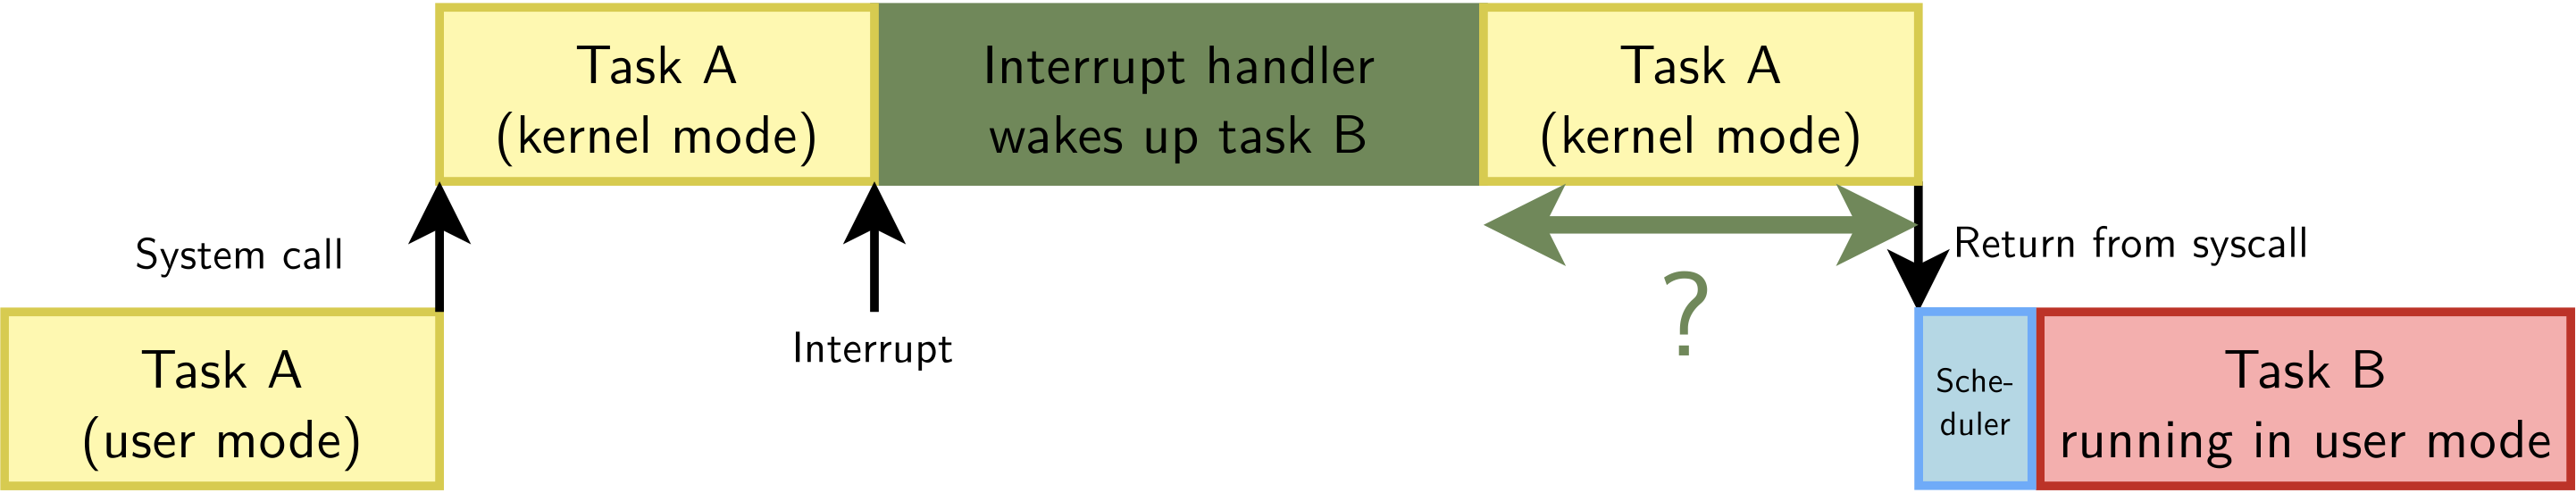
\includegraphics[width=1\textwidth]{assets/bootlin-interrupt-flow.png}
    \caption{From \cite{bootlinUnderstandingLinuxRealtime2024}, illustrating kernel-space latency from an interrupt in the Linux kernel.}
    \label{fig:bootlin_flow}
\end{figure}

\begin{figure}[H]
    \centering
    \begin{subfigure}{.49\textwidth}
        \centering
        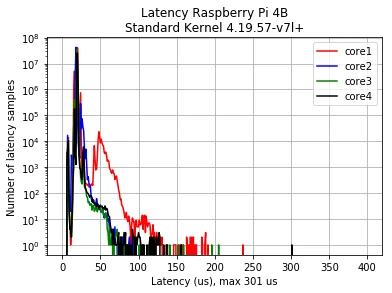
\includegraphics[width=1\linewidth]{assets/lemariva-std-kernel-latency.png}
        \caption{}
        \label{fig:std_latency}
    \end{subfigure}
    \hfill
    \begin{subfigure}{.49\textwidth}
        \centering
        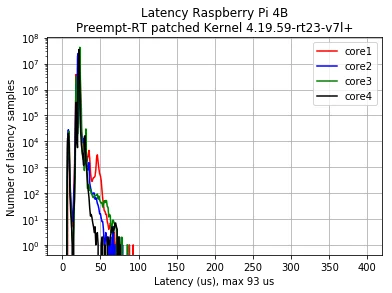
\includegraphics[width=1\linewidth]{assets/lemariva-rt-kernel-latency.png}
        \caption{}
        \label{fig:rt_latency}
    \end{subfigure}
    \caption{Latency measurements from \cite{maurorivaRaspberryPi4B2019} using Cyclictest from the RT-Tests suite. (\ref{sub@fig:std_latency}) The standard Linux RPi kernel, and (\ref{sub@fig:rt_latency}) the PREEMPT-RT kernel.}
    \label{fig:lemariva_latency}
\end{figure}

\subsubsection{Computing Platforms}
Field Programmable Gate Arrays (FPGAs), semiconductor devices structured around a matrix of configurable logic blocks (CLBs) interconnected via programmable interconnects \cite{WhatFPGAField}, are ideal solutions for computationally demanding image processing tasks, owing to their inherent hardware parallelism and low latency characteristics. Despite the availability of highly efficient intellectual property (IP) cores for FPGA-based logic acceleration, development and prototyping times may increase due to the intricate low-level hardware intricacies involved. Additionally, FPGAs typically incur higher costs compared to traditional CPU-based computing systems. On the other hand, the Raspberry Pi (RPi) company has been at the forefront of designing high-performance, cost-effective, single-board, and modular computers based on the Arm architecture and running the Linux operating system since 2012 \cite{raspberrypiltdRaspberryPiUs}. The standard RPi product lineup provides an excellent non-FPGA, CPU-based route for swift and straightforward development and deployment.

\subsubsection{Specialised Light Source}

A Digital Light Processing (DLP) projector plays a crucial role in projecting backscatter-cancelling light patterns. The DLP chipset comprises a Digital Micromirror Device (DMD), which houses millions of reflective aluminium mirrors, typically only a few microns wide. The DMD serves as a Micro-Opto-Electro-Mechanical System (MOEMS) Spatial Light Modulator (SLM), enabling the modulation and attenuation of an incident light beam with precision. As Figure \ref{fig:dmd_dlp} illustrates, a beam emitted from a high-intensity white lamp is directed towards a rotating colour-tinted lens wheel. Subsequently, an internal lens diffracts the coloured beam onto the DMD. The angle and duration of each microscopic mirror's activation dictate the intensity of individual pixels, redirecting the desired beams of each pixel through a diffraction lens to exit the projector. Inactive DMD mirrors direct the beam into a light-absorbing region to prevent light leakage and ensure image integrity.

\begin{figure}[H]
    \centering
    \begin{subfigure}{.4\textwidth}
        \centering
        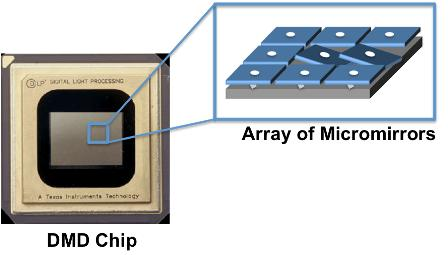
\includegraphics[width=1\linewidth]{assets/dmd-chip.jpg}
        \caption{}
        % \label{subfig:dmd_chip}
    \end{subfigure}
    % \hfill
    \hfill
    \begin{subfigure}{.49\textwidth}
        \centering
        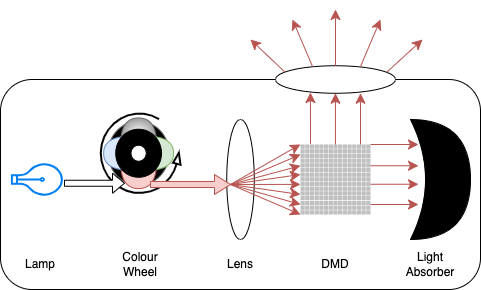
\includegraphics[width=1\linewidth]{assets/dlp-projector.png}
        \caption{}
        % \label{subfig:dlp_projector}
    \end{subfigure}
    \caption{(a) The microscopic mirror array within a DMD chip \cite{HowDoesDLP}. (b) Cross-sectional view of an example projector employing DLP technology.}
    \label{fig:dmd_dlp}
\end{figure}

\subsubsection{Specialised Camera Sensor}

The cameras found in many traditional and consumer-grade electronic devices, including smartphones, typically utilise a CMOS sensor equipped with a rolling shutter. These sensors introduce distortion effects when capturing fast-moving subjects, attributed to their line-by-line scan image-capturing characteristic. A global shutter sensor captures a snapshot of the scene using all pixels simultaneously, rather than line-by-line. Figures \ref{subfig:rs_timeline} and \ref{subfig:gs_timeline} depict the distinctions in image capture between a rolling shutter and a global shutter, and Figure \ref{subfig:rs_vs_gs} showcases capture differences. The Raspberry Pi company offers a global shutter camera with plug-and-play compatibility with Raspberry Pi computers.

\begin{figure}[H]
    \centering
    \begin{subfigure}{.45\textwidth}
        \centering
        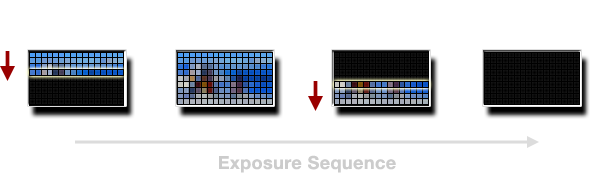
\includegraphics[width=1\linewidth]{assets/rolling-shutter-timeline.png}
        \caption{}
        \label{subfig:rs_timeline}
    \end{subfigure}
    \hfill
    \begin{subfigure}{.45\textwidth}
        \centering
        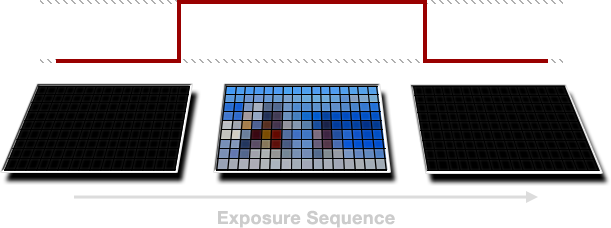
\includegraphics[width=1\linewidth]{assets/global-shutter-timeline.png}
        \caption{}
        \label{subfig:gs_timeline}
    \end{subfigure}
    \hfill
    \begin{subfigure}{0.45\textwidth}
        \centering
        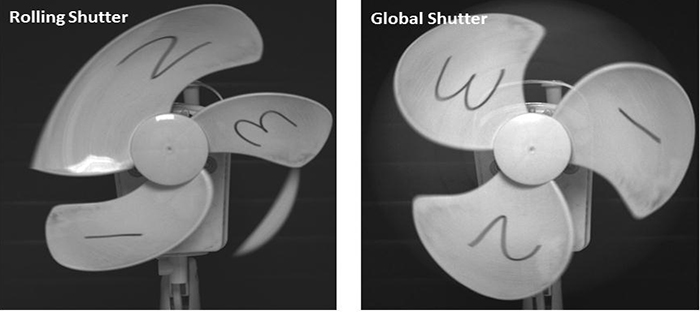
\includegraphics[width=0.7\textwidth]{assets/rolling-vs-global-shutter.jpeg}
        \caption{}
        \label{subfig:rs_vs_gs}
    \end{subfigure}
    \caption{The image capture of a rolling shutter sensor in (\ref{sub@subfig:rs_timeline}) and that of a global shutter in (\ref{sub@subfig:gs_timeline}) \cite{reddigitalcinemaGlobalRollingShutters}, and (\ref{sub@subfig:rs_vs_gs}), the comparison between the sensors when capturing a fast-moving target \cite{RollingShutterVs}.}
    \label{fig:rs_vs_gs}
\end{figure}

\subsection{Summary}
\label{bisummary}

From the background research, the best methodology for precise backscatter segmentation is the Canny edge detection approach due to its resilience in varying particle appearances, a limitation of Shepherd's simple blob detection approach, and robustness in detecting edges even in uneven illumination conditions, exemplified by Thomanek et al. drawing comparisons with simple image thresholding. Zelenka's use of the gradient-based Snake method, despite its capability to segment bubbles with bright spots inside them, is unnecessary for this project's objective, as the focus lies on eliminating just the backscatter within sediments, the bright spot within bubbles, sand, and other marine debris, rather than the entire sediment particle.

When considering the computing platform, a Raspberry Pi single-board computer (SBC) running a Linux OS, and developing the system with Python and OpenCV, is preferable over an FPGA for its cost-effectiveness, ease of development, and compatibility with a wide range of peripherals and software, aspects which are all essential for this project for prototyping in short time constraints. While a Raspberry Pi SBC that runs an ordinary Linux OS is not inherently a `hard' real-time system like an FPGA implementation, implementing the PREEMPT-RT Linux kernel patch offers improved determinism and reduced latency compared to a standard Linux OS, crucial for ensuring timely and predictable response in the system.

A DLP projector is the preferred choice for projecting backscatter-cancelling light patterns due to its precise control and modulation capabilities, essential for accurately overlaying patterns to eliminate backscatter. Opting for a global shutter camera sensor over a rolling shutter sensor mitigates distortion effects caused by fast-moving subjects, ensuring accurate image capture in dynamic underwater environments.
